\documentclass{beamer}\usepackage[]{graphicx}\usepackage[]{color}
%% maxwidth is the original width if it is less than linewidth
%% otherwise use linewidth (to make sure the graphics do not exceed the margin)
\makeatletter
\def\maxwidth{ %
  \ifdim\Gin@nat@width>\linewidth
    \linewidth
  \else
    \Gin@nat@width
  \fi
}
\makeatother

\definecolor{fgcolor}{rgb}{1, 0.894, 0.769}
\newcommand{\hlnum}[1]{\textcolor[rgb]{0.824,0.412,0.118}{#1}}%
\newcommand{\hlstr}[1]{\textcolor[rgb]{1,0.894,0.71}{#1}}%
\newcommand{\hlcom}[1]{\textcolor[rgb]{0.824,0.706,0.549}{#1}}%
\newcommand{\hlopt}[1]{\textcolor[rgb]{1,0.894,0.769}{#1}}%
\newcommand{\hlstd}[1]{\textcolor[rgb]{1,0.894,0.769}{#1}}%
\newcommand{\hlkwa}[1]{\textcolor[rgb]{0.941,0.902,0.549}{#1}}%
\newcommand{\hlkwb}[1]{\textcolor[rgb]{0.804,0.776,0.451}{#1}}%
\newcommand{\hlkwc}[1]{\textcolor[rgb]{0.78,0.941,0.545}{#1}}%
\newcommand{\hlkwd}[1]{\textcolor[rgb]{1,0.78,0.769}{#1}}%
\let\hlipl\hlkwb

\usepackage{framed}
\makeatletter
\newenvironment{kframe}{%
 \def\at@end@of@kframe{}%
 \ifinner\ifhmode%
  \def\at@end@of@kframe{\end{minipage}}%
  \begin{minipage}{\columnwidth}%
 \fi\fi%
 \def\FrameCommand##1{\hskip\@totalleftmargin \hskip-\fboxsep
 \colorbox{shadecolor}{##1}\hskip-\fboxsep
     % There is no \\@totalrightmargin, so:
     \hskip-\linewidth \hskip-\@totalleftmargin \hskip\columnwidth}%
 \MakeFramed {\advance\hsize-\width
   \@totalleftmargin\z@ \linewidth\hsize
   \@setminipage}}%
 {\par\unskip\endMakeFramed%
 \at@end@of@kframe}
\makeatother

\definecolor{shadecolor}{rgb}{.97, .97, .97}
\definecolor{messagecolor}{rgb}{0, 0, 0}
\definecolor{warningcolor}{rgb}{1, 0, 1}
\definecolor{errorcolor}{rgb}{1, 0, 0}
\newenvironment{knitrout}{}{} % an empty environment to be redefined in TeX

\usepackage{alltt}
\usepackage{../371g-slides}
\title{Multiple Regression}
\subtitle{Lecture 7}
\author{STA 371G}
\IfFileExists{upquote.sty}{\usepackage{upquote}}{}
\begin{document}
  
  
  

  \frame{\maketitle}

  % Show outline at beginning of each section
  \AtBeginSection[]{ 
    \begin{frame}<beamer>
      \tableofcontents[currentsection]
    \end{frame}
  }

  %%%%%%% Slides start here %%%%%%%

  \begin{darkframes}
  
  
    \begin{frame}
      How would you know how much to pay for a house? \pause
      
      Zillow? How do they know? 
      
      \begin{center}
        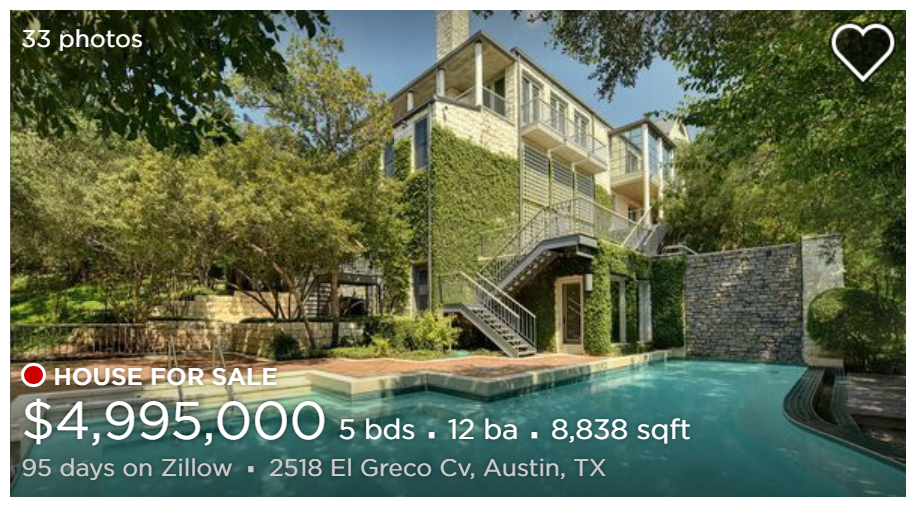
\includegraphics[width=3.5in]{zillow} \\
      \end{center} \pause
      
      \begin{columns}[onlytextwidth]
        \column{.5\textwidth}
          \begin{itemize}
            \item Square feet
            \item Year built
            \item \# of rooms
          \end{itemize}
        \column{.5\textwidth}
          \begin{itemize}
            \item Distance to downtown
            \item Crime rate
            \item Pollution
          \end{itemize}
      \end{columns}
      
      
    \end{frame}
    
    
    
    
    
    
    \begin{frame}
    
      \begin{center}
        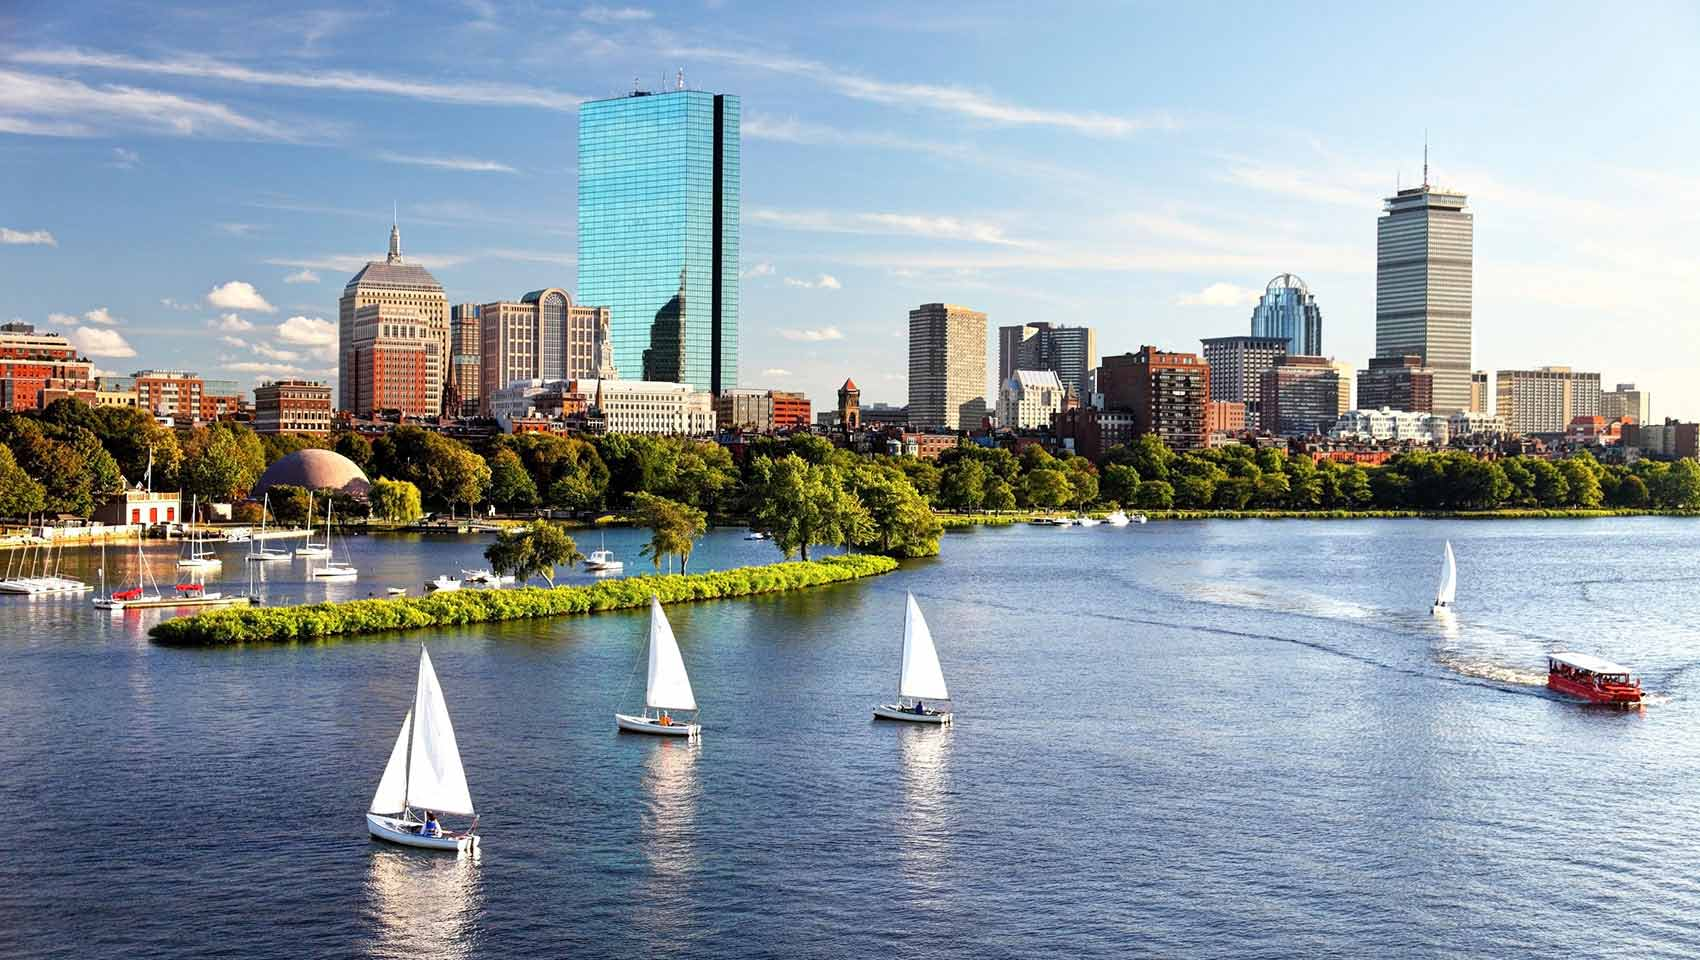
\includegraphics[width=4in]{boston} \\
      \end{center}
      
      Boston house price data (by census tract, 1970)
      \note{Every row corresponds to a census tract. The prices are multiplied by 20 to make them more relevant.}
    \end{frame}
    
    
    
    
    
    
    
    \begin{frame}
     
      \begin{columns}[onlytextwidth]
        \column{.5\textwidth}
          \begin{itemize}
            \item MEDV: Median Price (response)
            \item LONG: Longitude
            \item LAT: Latitude
            \item CRIME: Per capita crime rate
            \item ZONE: Proportion of large lots
            \item INDUS: Proportion of non-retail business acres
            \item NOX: Nitrogen Oxide concentration
          \end{itemize}
        \column{.5\textwidth}
          \begin{itemize}
            \item ROOM: Average \# of rooms
            \item AGE: Proportion of built before 1940
            \item DIST: Distance to employment centers
            \item RADIAL: Accessibility to highways
            \item TAX: Tax rate (per \$10K)
            \item PTRATIO: Pupil-to-teacher ratio
            \item LSTAT: Proportion of ``lower status''
            %  proportion of adults without some high school education or that are classified as laborers
          \end{itemize}
      \end{columns}
    
    \end{frame}
    
    
    
    
    
    \begin{frame}
        Can you guess top three factors?
        \lc
    \end{frame}
    
    
    
    
    \begin{frame}[fragile]{Distribution of house prices (MEDV)}
      \fontsize{10}{10}\selectfont
\begin{knitrout}
\definecolor{shadecolor}{rgb}{0.137, 0.137, 0.137}\begin{kframe}
\begin{alltt}
\hlstd{> }\hlkwd{hist}\hlstd{(boston}\hlopt{$}\hlstd{MEDV,} \hlkwc{col}\hlstd{=}\hlstr{'green'}\hlstd{,}
\hlstd{+ }  \hlkwc{main}\hlstd{=}\hlstr{''}\hlstd{,} \hlkwc{xlab}\hlstd{=}\hlstr{'Census Tract Median House Price'}\hlstd{)}
\end{alltt}
\end{kframe}
\input{C:/temp/figures/unnamed-chunk-3-1.tikz}

\end{knitrout}
      \note{Not a normal distribution... We can mention log-normal distributions.}
    \end{frame}
    
    
        \begin{frame}{Multiple Regression Model}
      
      We model the median price in a census tract ($y_i=$ median price in $i$th tract) as a linear function of multiple predictors, plus some error.
      
      \[
        y_i = \beta_0 + \beta_1 x_{i1} + \beta_2 x_{i2} +\ldots + \beta_{13} x_{i13} + \epsilon_i
      \]
      
    \begin{table}[!b]
        {\carlitoTLF % Use monospaced lining figures
        \begin{tabularx}{\textwidth}{Xrrrrrr}
           
           & $\beta_0$ & $\beta_1$ & \beta_2 & \textbf{...} &   \beta_{13} & \\
          \toprule

          & & \textbf{LAT} & \textbf{LON} & \textbf{...} &   \textbf{LSTAT} & \textbf{error}\\
          \toprule
    $y_1$ & 1 & $x_{11}$ & $x_{12}$  & \textbf{...} & $x_{1,13}$ & $\epsilon_1$  \\
    $y_2$ & 1 & $x_{21}$ & $x_{22}$  & \textbf{...} & $x_{2,13}$ & $\epsilon_2$\\
    \textbf{...}  & \textbf{...} &  \textbf{...} & \textbf{...}  & \textbf{...} &   \textbf{...}  & \textbf{...}\\
    %$y_{503}$ & 1 &  $x_{503,1}$ & $x_{503,2}$  & \textbf{...} &   $x_{503,13}$  & $\epsilon_{503}$\\
      
          \bottomrule
        \end{tabularx}}
        
      \end{table}     
     
      \bigskip\pause
      
      We find $\hat\beta_0,\ldots,\hat\beta_{13}$ to minimize the residuals ($\hat y_i - y_i$)
      
      %\[
      %  \hat y_i = \hat\beta_0 + \hat\beta_1 x_{i1} + \hat\beta_2 x_{i2} +\ldots + \hat\beta_{13} x_{i13} 
      %\]
    \end{frame}
    
    
  
  
  
    \begin{frame}[fragile]
      \fontsize{9}{9}\selectfont
\begin{knitrout}
\definecolor{shadecolor}{rgb}{0.137, 0.137, 0.137}\begin{kframe}
\begin{alltt}
\hlstd{> }\hlstd{model} \hlkwb{<-} \hlkwd{lm}\hlstd{(MEDV} \hlopt{~} \hlstd{LON}\hlopt{+}\hlstd{LAT}\hlopt{+}\hlstd{CRIME}\hlopt{+}\hlstd{ZONE}\hlopt{+}\hlstd{INDUS}\hlopt{+}\hlstd{NOX}\hlopt{+}\hlstd{ROOM}\hlopt{+}\hlstd{AGE}\hlopt{+}\hlstd{DIST}
\hlstd{+ }                  \hlopt{+}\hlstd{RADIAL}\hlopt{+}\hlstd{TAX}\hlopt{+}\hlstd{PTRATIO}\hlopt{+}\hlstd{LSTAT,} \hlkwc{data}\hlstd{=boston)}
\hlstd{> }\hlkwd{summary}\hlstd{(model}\hlopt{$}\hlstd{residuals)}
\end{alltt}
\begin{verbatim}
   Min. 1st Qu.  Median    Mean 3rd Qu.    Max. 
-258.10  -57.34  -13.64    0.00   39.61  531.30 
\end{verbatim}
\begin{alltt}
\hlstd{> }\hlkwd{summary}\hlstd{(model)}\hlopt{$}\hlstd{r.squared}
\end{alltt}
\begin{verbatim}
[1] 0.7305487
\end{verbatim}
\begin{alltt}
\hlstd{> }\hlkwd{summary}\hlstd{(model)}\hlopt{$}\hlstd{adj.r.squared}
\end{alltt}
\begin{verbatim}
[1] 0.7234291
\end{verbatim}
\end{kframe}
\end{knitrout}
      This is a high $R^2$ compared to the prior examples!
      
      Keep an eye on the Adjusted-$R^2$...
    \end{frame}
    
    
    \begin{frame}[fragile]
      Here is how the predictors contribute to the estimation:
      \fontsize{9}{9}\selectfont
\begin{knitrout}
\definecolor{shadecolor}{rgb}{0.137, 0.137, 0.137}\begin{kframe}
\begin{alltt}
\hlstd{> }\hlkwd{round}\hlstd{(}\hlkwd{summary}\hlstd{(model)}\hlopt{$}\hlstd{coefficients,}\hlnum{3}\hlstd{)}
\end{alltt}
\begin{verbatim}
              Estimate Std. Error t value Pr(>|t|)
(Intercept) -10815.107   6202.196  -1.744    0.082
LON           -100.538     68.540  -1.467    0.143
LAT            105.814     75.440   1.403    0.161
CRIME           -2.498      0.666  -3.752    0.000
ZONE             0.921      0.283   3.257    0.001
INDUS            0.448      1.267   0.353    0.724
NOX           -320.021     82.010  -3.902    0.000
ROOM            72.906      8.530   8.547    0.000
AGE              0.167      0.273   0.612    0.541
DIST           -27.490      4.296  -6.399    0.000
RADIAL           6.274      1.363   4.604    0.000
TAX             -0.287      0.076  -3.770    0.000
PTRATIO        -18.304      2.802  -6.533    0.000
LSTAT          -11.416      1.022 -11.169    0.000
\end{verbatim}
\end{kframe}
\end{knitrout}
      \quad \pause
      
      INDUS, AGE, LAT and LON seem to be statistically insignificant. Should we omit them altogether?
    \end{frame}
    
    
    
    
    \begin{frame}
      P-value of a predictor shown in the summary is in the \alert{marginal} sense! 
      
      \bigskip
      
      Omitting other predictors might increase the significance (decrease the P-value) of a statistically insignificant predictor.
    \end{frame}

    
    \begin{frame}[fragile]
      \fontsize{9}{9}\selectfont
\begin{knitrout}
\definecolor{shadecolor}{rgb}{0.137, 0.137, 0.137}\begin{kframe}
\begin{alltt}
\hlstd{> }\hlstd{model_red} \hlkwb{<-} \hlkwd{lm}\hlstd{(MEDV} \hlopt{~} \hlstd{LON}\hlopt{+}\hlstd{LAT}\hlopt{+}\hlstd{INDUS}\hlopt{+}\hlstd{AGE,} \hlkwc{data}\hlstd{=boston)}
\hlstd{> }\hlkwd{round}\hlstd{(}\hlkwd{summary}\hlstd{(model_red)}\hlopt{$}\hlstd{coefficients,}\hlnum{3}\hlstd{)}
\end{alltt}
\begin{verbatim}
              Estimate Std. Error t value Pr(>|t|)
(Intercept) -54327.834   8559.058  -6.347    0.000
LON           -709.317     92.859  -7.639    0.000
LAT            107.180    111.630   0.960    0.337
INDUS          -11.818      1.305  -9.052    0.000
AGE             -0.236      0.324  -0.727    0.468
\end{verbatim}
\begin{alltt}
\hlstd{> }\hlkwd{summary}\hlstd{(model_red)}\hlopt{$}\hlstd{r.squared}
\end{alltt}
\begin{verbatim}
[1] 0.3203884
\end{verbatim}
\end{kframe}
\end{knitrout}
      LON and INDUS look like a big deal now, although they do not explain as much with $R^2=0.32$.
      
      Let's start omiting one by one.
    \end{frame}
    
    
    
    
    \begin{frame}[fragile]
      \fontsize{9}{9}\selectfont
      INDUS has been omitted.
\begin{knitrout}
\definecolor{shadecolor}{rgb}{0.137, 0.137, 0.137}\begin{kframe}
\begin{alltt}
\hlstd{> }\hlstd{model} \hlkwb{<-} \hlkwd{lm}\hlstd{(MEDV} \hlopt{~} \hlstd{LON}\hlopt{+}\hlstd{LAT}\hlopt{+}\hlstd{CRIME}\hlopt{+}\hlstd{ZONE}\hlopt{+}\hlstd{NOX}\hlopt{+}\hlstd{ROOM}\hlopt{+}\hlstd{AGE}\hlopt{+}\hlstd{DIST}
\hlstd{+ }                  \hlopt{+}\hlstd{RADIAL}\hlopt{+}\hlstd{TAX}\hlopt{+}\hlstd{PTRATIO}\hlopt{+}\hlstd{LSTAT,} \hlkwc{data}\hlstd{=boston)}
\hlstd{> }\hlkwd{summary}\hlstd{(model)}\hlopt{$}\hlstd{r.squared}
\end{alltt}
\begin{verbatim}
[1] 0.7304803
\end{verbatim}
\begin{alltt}
\hlstd{> }\hlkwd{summary}\hlstd{(model)}\hlopt{$}\hlstd{adj.r.squared}
\end{alltt}
\begin{verbatim}
[1] 0.72392
\end{verbatim}
\end{kframe}
\end{knitrout}
      $R^2$ has not changed too much, Adjusted-$R^2$ has increased a bit.
    \end{frame}
    
    
    \begin{frame}[fragile]
      \fontsize{9}{9}\selectfont
\begin{knitrout}
\definecolor{shadecolor}{rgb}{0.137, 0.137, 0.137}\begin{kframe}
\begin{alltt}
\hlstd{> }\hlkwd{round}\hlstd{(}\hlkwd{summary}\hlstd{(model)}\hlopt{$}\hlstd{coefficients,}\hlnum{3}\hlstd{)}
\end{alltt}
\begin{verbatim}
              Estimate Std. Error t value Pr(>|t|)
(Intercept) -11078.359   6151.843  -1.801    0.072
LON           -104.687     67.467  -1.552    0.121
LAT            104.977     75.335   1.393    0.164
CRIME           -2.504      0.665  -3.766    0.000
ZONE             0.908      0.280   3.242    0.001
NOX           -311.363     78.196  -3.982    0.000
ROOM            72.587      8.474   8.566    0.000
AGE              0.171      0.273   0.626    0.531
DIST           -27.725      4.240  -6.539    0.000
RADIAL           6.137      1.305   4.703    0.000
TAX             -0.275      0.069  -4.005    0.000
PTRATIO        -18.137      2.759  -6.573    0.000
LSTAT          -11.391      1.019 -11.182    0.000
\end{verbatim}
\end{kframe}
\end{knitrout}
    
      
      AGE still seems insignificant.
    \end{frame}
    
    
    
    
    
    \begin{frame}[fragile]
      \fontsize{9}{9}\selectfont
      AGE has been omitted.
\begin{knitrout}
\definecolor{shadecolor}{rgb}{0.137, 0.137, 0.137}\begin{kframe}
\begin{alltt}
\hlstd{> }\hlstd{model} \hlkwb{<-} \hlkwd{lm}\hlstd{(MEDV} \hlopt{~} \hlstd{LON}\hlopt{+}\hlstd{LAT}\hlopt{+}\hlstd{CRIME}\hlopt{+}\hlstd{ZONE}\hlopt{+}\hlstd{NOX}\hlopt{+}\hlstd{ROOM}\hlopt{+}\hlstd{DIST}
\hlstd{+ }                  \hlopt{+}\hlstd{RADIAL}\hlopt{+}\hlstd{TAX}\hlopt{+}\hlstd{PTRATIO}\hlopt{+}\hlstd{LSTAT,} \hlkwc{data}\hlstd{=boston)}
\hlstd{> }\hlkwd{summary}\hlstd{(model)}\hlopt{$}\hlstd{r.squared}
\end{alltt}
\begin{verbatim}
[1] 0.7302658
\end{verbatim}
\begin{alltt}
\hlstd{> }\hlkwd{summary}\hlstd{(model)}\hlopt{$}\hlstd{adj.r.squared}
\end{alltt}
\begin{verbatim}
[1] 0.7242596
\end{verbatim}
\end{kframe}
\end{knitrout}
      $R^2$ is again about the same, and Adjusted-$R^2$ has increased a bit.
    \end{frame}
    
    
    \begin{frame}[fragile]
      \fontsize{9}{9}\selectfont
\begin{knitrout}
\definecolor{shadecolor}{rgb}{0.137, 0.137, 0.137}\begin{kframe}
\begin{alltt}
\hlstd{> }\hlkwd{round}\hlstd{(}\hlkwd{summary}\hlstd{(model)}\hlopt{$}\hlstd{coefficients,}\hlnum{3}\hlstd{)}
\end{alltt}
\begin{verbatim}
              Estimate Std. Error t value Pr(>|t|)
(Intercept) -10647.181   6109.452  -1.743    0.082
LON            -97.364     66.406  -1.466    0.143
LAT            107.052     75.216   1.423    0.155
CRIME           -2.513      0.664  -3.782    0.000
ZONE             0.891      0.279   3.199    0.001
NOX           -300.532     76.214  -3.943    0.000
ROOM            73.744      8.265   8.922    0.000
DIST           -28.594      4.004  -7.141    0.000
RADIAL           6.089      1.302   4.677    0.000
TAX             -0.274      0.069  -3.986    0.000
PTRATIO        -18.104      2.757  -6.566    0.000
LSTAT          -11.178      0.959 -11.651    0.000
\end{verbatim}
\end{kframe}
\end{knitrout}
      LAT is next.
    \end{frame}
    
    
    
    \begin{frame}[fragile]
      \fontsize{9}{9}\selectfont
      LAT has been omitted.
\begin{knitrout}
\definecolor{shadecolor}{rgb}{0.137, 0.137, 0.137}\begin{kframe}
\begin{alltt}
\hlstd{> }\hlstd{model} \hlkwb{<-} \hlkwd{lm}\hlstd{(MEDV} \hlopt{~} \hlstd{LON}\hlopt{+}\hlstd{CRIME}\hlopt{+}\hlstd{ZONE}\hlopt{+}\hlstd{NOX}\hlopt{+}\hlstd{ROOM}\hlopt{+}\hlstd{DIST}
\hlstd{+ }                  \hlopt{+}\hlstd{RADIAL}\hlopt{+}\hlstd{TAX}\hlopt{+}\hlstd{PTRATIO}\hlopt{+}\hlstd{LSTAT,} \hlkwc{data}\hlstd{=boston)}
\hlstd{> }\hlkwd{summary}\hlstd{(model)}\hlopt{$}\hlstd{r.squared}
\end{alltt}
\begin{verbatim}
[1] 0.7291597
\end{verbatim}
\begin{alltt}
\hlstd{> }\hlkwd{summary}\hlstd{(model)}\hlopt{$}\hlstd{adj.r.squared}
\end{alltt}
\begin{verbatim}
[1] 0.7236882
\end{verbatim}
\end{kframe}
\end{knitrout}
      Both $R^2$ and Adjusted-$R^2$ have reduced. But still not too bad.
    \end{frame}
    
    
    \begin{frame}[fragile]
      \fontsize{9}{9}\selectfont
\begin{knitrout}
\definecolor{shadecolor}{rgb}{0.137, 0.137, 0.137}\begin{kframe}
\begin{alltt}
\hlstd{> }\hlkwd{round}\hlstd{(}\hlkwd{summary}\hlstd{(model)}\hlopt{$}\hlstd{coefficients,}\hlnum{3}\hlstd{)}
\end{alltt}
\begin{verbatim}
             Estimate Std. Error t value Pr(>|t|)
(Intercept) -5072.211   4693.369  -1.081    0.280
LON           -82.750     65.675  -1.260    0.208
CRIME          -2.507      0.665  -3.770    0.000
ZONE            0.874      0.279   3.137    0.002
NOX          -318.435     75.247  -4.232    0.000
ROOM           73.595      8.273   8.896    0.000
DIST          -29.692      3.933  -7.549    0.000
RADIAL          5.854      1.293   4.529    0.000
TAX            -0.272      0.069  -3.955    0.000
PTRATIO       -18.212      2.759  -6.601    0.000
LSTAT         -11.062      0.957 -11.560    0.000
\end{verbatim}
\end{kframe}
\end{knitrout}
      Bye LON...
    \end{frame}
    
    
    \begin{frame}[fragile]
      \fontsize{9}{9}\selectfont
      LON has been omitted.
\begin{knitrout}
\definecolor{shadecolor}{rgb}{0.137, 0.137, 0.137}\begin{kframe}
\begin{alltt}
\hlstd{> }\hlstd{model} \hlkwb{<-} \hlkwd{lm}\hlstd{(MEDV} \hlopt{~} \hlstd{CRIME}\hlopt{+}\hlstd{ZONE}\hlopt{+}\hlstd{NOX}\hlopt{+}\hlstd{ROOM}\hlopt{+}\hlstd{DIST}
\hlstd{+ }                  \hlopt{+}\hlstd{RADIAL}\hlopt{+}\hlstd{TAX}\hlopt{+}\hlstd{PTRATIO}\hlopt{+}\hlstd{LSTAT,} \hlkwc{data}\hlstd{=boston)}
\hlstd{> }\hlkwd{summary}\hlstd{(model)}\hlopt{$}\hlstd{r.squared}
\end{alltt}
\begin{verbatim}
[1] 0.7282911
\end{verbatim}
\begin{alltt}
\hlstd{> }\hlkwd{summary}\hlstd{(model)}\hlopt{$}\hlstd{adj.r.squared}
\end{alltt}
\begin{verbatim}
[1] 0.7233609
\end{verbatim}
\end{kframe}
\end{knitrout}
      Both $R^2$ and Adjusted-$R^2$ have reduced. But that's OK.
    \end{frame}
    
    
    \begin{frame}[fragile]
      \fontsize{9}{9}\selectfont
\begin{knitrout}
\definecolor{shadecolor}{rgb}{0.137, 0.137, 0.137}\begin{kframe}
\begin{alltt}
\hlstd{> }\hlkwd{round}\hlstd{(}\hlkwd{summary}\hlstd{(model)}\hlopt{$}\hlstd{coefficients,}\hlnum{3}\hlstd{)}
\end{alltt}
\begin{verbatim}
            Estimate Std. Error t value Pr(>|t|)
(Intercept)  840.065     99.001   8.485    0.000
CRIME         -2.566      0.664  -3.866    0.000
ZONE           0.922      0.276   3.338    0.001
NOX         -346.926     71.811  -4.831    0.000
ROOM          74.243      8.262   8.986    0.000
DIST         -31.050      3.785  -8.203    0.000
RADIAL         6.000      1.288   4.658    0.000
TAX           -0.265      0.069  -3.870    0.000
PTRATIO      -19.280      2.627  -7.339    0.000
LSTAT        -11.072      0.957 -11.563    0.000
\end{verbatim}
\end{kframe}
\end{knitrout}
      Notice what happened to the intercept. LON (and perhaps the others) was acting like an intercept!
    \end{frame}
    
    
    \begin{frame}{When to omit, when to keep?}
      We often prefer to omit statistically insignificant variables. Because:
      \begin{itemize}
        \item The model gets simpler.
        \item Insignificant variables may lead to incorrect interpretations (as in LON).
        \item Especially when data is small, insignificant variables harm the quality of the model.
        
      \end{itemize}
      
    \end{frame}
    
    \begin{frame}{When to omit, when to keep?}
      We often prefer to omit statistically insignificant variables. Because:
      \begin{itemize}
        \item The model gets simpler.
        \item Insignificant variables may lead to incorrect interpretations (as in LON).
        \item Especially when data is small, insignificant variables harm the quality of the model.
        
      \end{itemize}
      
    \end{frame}
    
 
  \end{darkframes}

\end{document}
